\documentclass[paper=A4,pagesize,DIV=18, 12pt,listof=totoc,bibliography=totoc,headings=optiontohead,open=any]{article}
\usepackage[utf8]{inputenc}
\usepackage[T1]{fontenc}
\usepackage[ngerman]{babel}
\usepackage[babel,german=quotes]{csquotes}
\usepackage{siunitx}
\sisetup{locale = DE}
\usepackage[pdftex]{graphicx}
\usepackage{cleveref}
\pdfcompresslevel=0
\DeclareGraphicsExtensions{.png,.jpg,.pdf,.gif}

\usepackage[backend=bibtex]{biblatex}
\bibliography{quellen.bib}

\usepackage{epstopdf}
\usepackage{float}
\usepackage{caption}
\usepackage{subcaption}
\usepackage{tikz}
\usepackage{tikz-3dplot}
\usepackage{pdfpages}
\usepackage{setspace}
\usepackage{glossaries}

\usepackage{amsmath}



\date{\today}
\author{Philipp Hörauf, Toni Bartsch}
\title{DIY: Die Carbonwickelmaschine}

\begin{document}
\maketitle
\thispagestyle{empty}
\vspace*{15mm}
\begin{figure}[H]
	\centering
	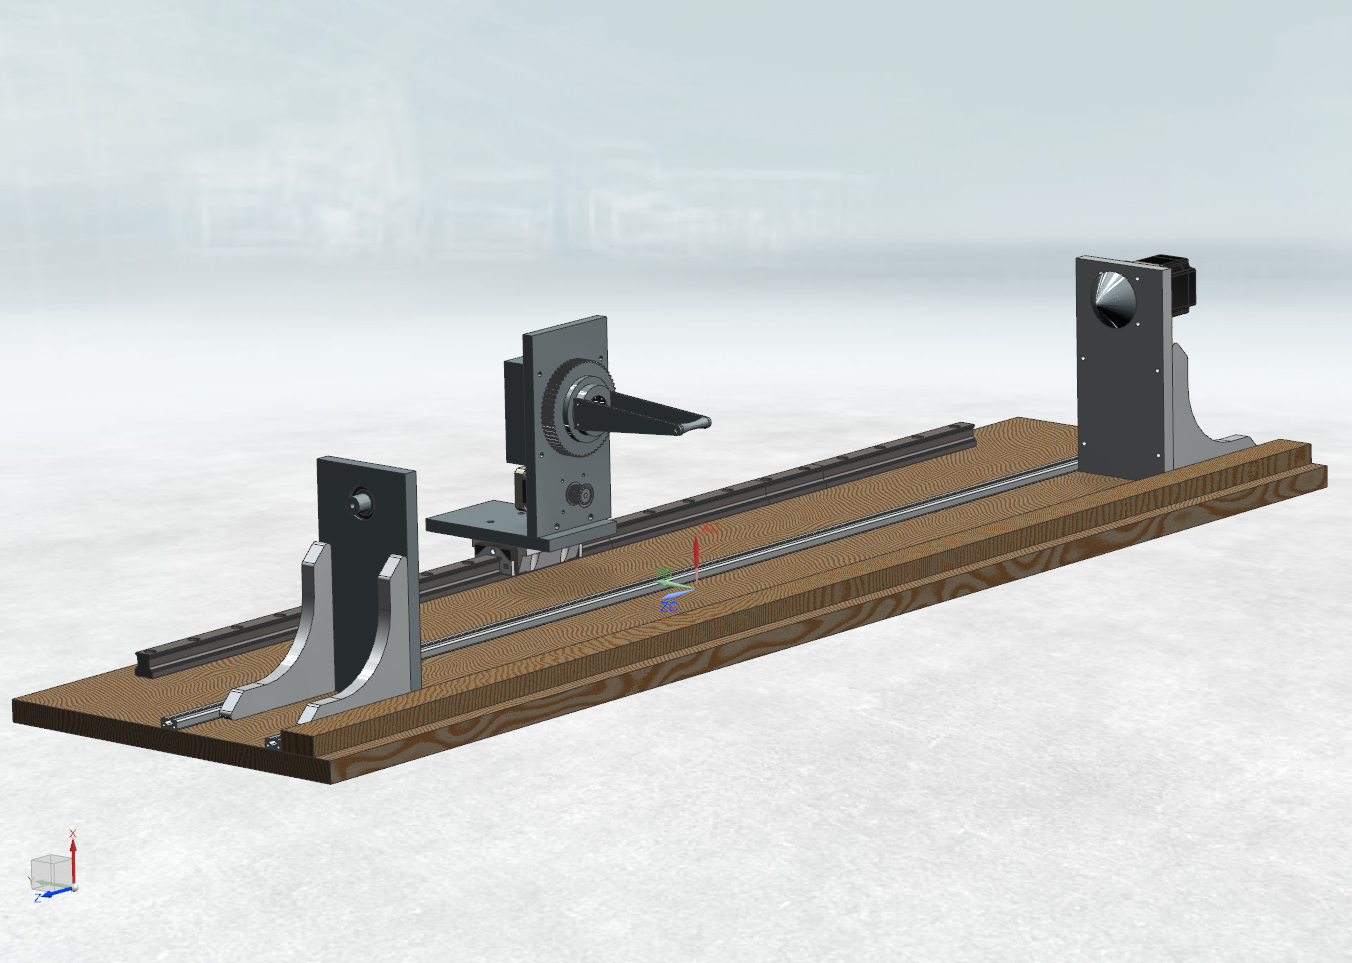
\includegraphics[width=1\textwidth]{NX_Screenshots/gesamt3.png}
\end{figure}

\pagenumbering{Roman}

\newpage
\tableofcontents
\newpage

% ab hier normale Zeilennummern.
\pagenumbering{arabic}
\section{Einleitung}
Ziel des Projektes ist eine Carbonwickelmaschine zu entwickeln um zylindrische und konische Wickelkörper mit unterschiedlichen Rovings bewickeln zu können. Auf diese Weise soll es möglich sein extrem leichte, verschwindungssteife und korrosionsbeständig Rohre herzustellen die quasi immun gegen Wärmeausdehnung sind. Für diesen Zweck gibt es zwar bereits Maschinen, die aber entweder für deutlich größere Teile ausgelegt sind, oder die sehr teuer bzw. nicht als Bauplan kostenlos verfügbar sind.

\section{Spezifikationen und Überblick}
Die geplanten Spezifikationen für die Maschine sind:

\begin{itemize}
    \item Maximale Wickellänge \SI{1200}{\milli\metre}
    \item Größter Durchmesser des Wickelkörpers \SI{250}{\milli\metre}
    \item Verarbeitung von Carbon- und Glasfasern
    \item Wickelvorgang PC-gesteuert
    \item Möglichst kostengünstiger Aufbau
    \item Konstruktion und Fertigung der Maschine aus Aluminium und Holz
    \item Vier Achsen, davon zwei mal Rotation und zwei mal Linear
\end{itemize}

\subsection{Elektronik}
\begin{itemize}
    \item Vier Schrittmotoren
    \item GRBL-Board 
    \item Netzteil
    \item Endschalter
\end{itemize}


\subsection{Software}
\begin{itemize}
    \item G-Code Generator mit graphischem Userinterface und einstellbaren Parametern
    \item GRBL Interface zum streamen des G-Codes und manuellem Verfahren
    \item GRBL auf einem Arduino, zur Ansteuerung der Schrittmotortreiber
\end{itemize}

\section{Grundlagen}
Um die Funktionsweise und den Aufbau der Wickelmaschine besser verstehen zu können sollen als erstes einige wichtige Grundlagen zu den verwendeten Faserverbundwerkstoffen sowie dem Wickelvorgang erklärt werden. Die Wickelmaschine arbeitet grundsätzlich nach dem Prinzip, dass eine Form, z.B. ein Rohr mit einem Faserverbundwerkstoff umwickelt wird. Je nach Form und Vorbehandlung verbleibt die Form im fertigen Teil, oder wird wieder entfernt. Im Folgenden sollen zuerst die Faserwerkstoffe näher betrachtet werden.

\subsection{Faserverbundwerkstoffe}
Faserverbundwerkstoffe werden durch Zusammenfügen mehrerer Werkstoffe hergestellt, zum einen aus einer formgebenden Matrix und zum anderen aus den verstärkenden Fasern. Als Matrix werden häufig Epoxyd- oder Polyesterharze verwendet, als Faserwerkstoffe Glas-, Kohlenstoff- oder Aramidfasern. Eine wichtige Eigenschaft der Faserverbundwerkstoffe ist die richtungsabhängige Festigkeit. Allgemein gilt, dass die Stabilität der Fasern in Längsrichtung um ein vielfaches höher ist als bei Scherkräften. Die Faserrichtung ist somit bei Konstruktion und Fertigung auf jeden Fall zu beachten.  Die folgende Übersicht soll einen Überblick über die wichtigsten Vor- und Nachteile der verschiedenen Fasern und Harze bieten und so die Entscheidungsfindung je nach Anwendungsfall erleichtern. \cite{r_g_wiki}

\begin{itemize}
	\item Epoxydharz Vorteile
	\begin{itemize}
		\item Hohe statische und dynamische Festigkeit
		\item Geringer Härtungsschwund, gute Maßhaltigkeit
		\item Hohe Temperaturbeständigkeit
		\item Gute Chemikalien- und Witterungsbeständigkeit
		\item Geringe Brennbarkeit
	\end{itemize}
	\item Epoxydharz Nachteile
	\begin{itemize}
		\item Hoher Preis
		\item Genaues Dosieren der Komponenten erforderlich
	\end{itemize}
	\item Polyesterharz Vorteile	
	\begin{itemize}
		\item Vergleichsweise günstig
		\item Anschleifen beim Überlaminieren meist nicht erforderlich
	\end{itemize} 
	\item Polyesterharz Nachteile
	\begin{itemize}
		\item Hoher Härtungsschwund
		\item Starker Styrolgeruch beim Verarbeiten
		\item Bei Verarbeitung ohne Sauerstoffausschluss leicht klebrige, riechende Oberfläche. Dadurch weniger Chemikalien- und Witterungsbeständig als Epoxydharz
	\end{itemize}	 
\end{itemize}

Zusammenfassend ist zu sagen, dass Epoxydharz gegenüber Polyesterharz die besseren technischen Eigenschaften aufweist, dafür aber deutlich teurer ist. Da hier aber die Witterungsbeständigkeit und die geringere Schrumpfung wichtig sind, wird Epoxydharz verwendet. Durch die geringere Schrumpfung ist in diesem Fall insbesondere ein leichteres Entformen zu erwarten.

Sowohl Epoxydharz- als auch Polyesterharzsysteme gibt es mit unterschiedlich Topf- bzw. Verarbeitungszeiten. Auch zu beachten ist, dass es Harze mit unterschiedlichen Anforderungen an die Bedingungen beim Härten gibt, insbesondere bzgl. Temperatur und Druck. Hier sollte ein passendes Produkt ausgewählt werden. In unserem Fall sind das Harze, die bereits bei Raumtemperatur vollständig aushärten.

Im Folgenden werden die häufig verwendete Kohle- und Glasfaser verglichen. Darüber hinaus gibt es noch weitere wie Aramid oder verschiedene Naturfasern, die hier allerdings keine Anwendung finden und deswegen auch nicht weiter erwähnt werden.

\begin{itemize}
	\item Kohlefaser
	\begin{itemize}
		\item Sehr hohe Zugfestigkeit
		\item Elektrisch leitend
		\item Gute Tränkungseigenschaften
		\item Vergleichsweise teuer
	\end{itemize}
	\item Glasfaser
	\begin{itemize}
		\item Etwas geringere Zugfestigkeit als Kohlefaser
		\item Elektrisch nicht leitend
		\item Teilweise schlechtere Tränkungseigenschaften
		\item Deutlich günstiger als Kohlefaser
		\item Bei gleicher Stabilität schwerer als Kohlefaser
	\end{itemize}
\end{itemize}

Die Entscheidung zwischen Kohlefaser und Glasfaser ist je nach Anwendung abzuwägen. Spielt das Gewicht eine eher geringe Rolle ist tendenziell Glasfaser aufgrund des günstigeren Preises zu bevorzugen. 
In Abbildung \ref{fig:roving} ist einer der verwendeten Kohlefaserrovings abgebildet. \cite{r_g_handbuch}
\begin{figure}[H]
	\centering
	\includegraphics[width=0.8\textwidth]{bilder/IMG_2629.JPG}
	\caption{Kohlefaserroving} 
	\label{fig:roving}
\end{figure}

%Quelle R&G_Handbuch.pdf
%Quelle: http://www.r-g.de/wiki/Was_sind_Faserverbundwerkstoffe%3F



\subsection{Die Mathematik des Wickelns}
\label{mathematik}
Um die gewünschten Wickelmuster zu erzeugen ist es wichtig, dieses zuerst mathematisch zu beschreiben. Dies geht am besten im Zylinderkoordinatensystem, wobei die Länge $r$ konstant bleibt und der Winkel $\varphi$ ständig inkrementiert wird, so lange sich der Wickelkörper dreht und damit den Roving aufwickelt. Der Schlitten verfährt dabei in z-Richtung. Dazu ist es nötig die Steigung $s(z)$ der Windung als Weg pro Umdrehung zu definieren. Es gibt für eine komplette Windung, also von $z = 0$ bis $z = z_{max}$ mehrere Zustände des Wickelns.\\
\begin{itemize}
	\item Anfangsstück: Bereich von $z = 0$ bis $z = z_{start}$
	\item Mitte: Bereich von $z = z_{start}$ bis $z = z_{end}$
	\item Endstück: Bereich von $z = z_{end}$ bis $z = z_{max}$
\end{itemize}
In den drei Abschnitten muss jeweils auf die Steigung eingegangen werden, diese ist nur in der Mitte konstant und lässt sich auch nur hier aus dem vorgegeben Wickelwinkel bestimmen, an den übrigen beiden Stücken ist die Steigung von $z$ abhängig. Das kommt daher, dass eine Windung bei $z = 0$ und $s = 0$ anfängt, da die Steigung beim Umkehren kurzzeitig Null wird und das Umkehren immer bei $z = 0$ und $z = z_{max}$ geschieht. Der Wickelvorgang selbst ist im Zylinderkoordinatensystem durch einen linear steigenden Winkel $\varphi$ und ein abschnittsweise definiertes $s(z)$ zu berechnen. Für den Wickelgang \enquote{vorwärts} ist $s = s(z)$ und rückwärts ist $s = -s(z)$. $s(z)$ muss unbedingt auf dem gesamten Bereich $z \in [0; z_{max}]$ stetig sein, da die Steigung beim Wickeln nicht springen kann, dazu müsste der Roving reißen oder umgesetzt werden, was schlicht physikalisch nicht geht.\\
Komplizierter wird es nun, wenn die Längen von Anfangs- und Endstück nicht gleich sind, da dann die Steigung am Anfang einer anderen Abhängigkeit folgt, als am Ende, um die Stetigkeit von $s$ garantieren zu können. Im einfachsten Falle (Abhängigkeit rein linear) ist $s(z)$ eine lineare Funktion, die die sich aus den Punkten $s(z = 0)$, $s(z = z_{start}$ und $z = z_{max}$ berechnen lässt.\\
\begin{equation}\label{steigungHin}
	s(z)=
	\begin{cases}
		\frac{z}{z_{start}} \cdot s_{soll} & \text{für } z \leq z_{start}\\
		s_{soll} & \text{für } z_{start} \leq z \leq z_{end}\\
		\left( 1 - \frac{z}{z_{max}}\right) \cdot s_{soll} & \text{für } z \leq z_{max}
	\end{cases}	
\end{equation}\\
Damit ist jetzt die Steigung für alle möglichen Fälle definiert, so lange sie sich nur linear verändern darf. Für eine anderweitige Abhängigkeit, Beispielsweise eine exponentielle zu- und Abnahme der Steigung ist die obrige Funktion entsprechend anzupassen. Für die ersten Tests wird darauf jedoch verzichtet und eine rein linaere Funktion gewählt.\\
Eine weitere Schwierigkeit besteht darin, den Roving nach jedem Durchgang zielgenau und mit einem definierten Versatz zum vorherigen Durchgang auf das Rohr aufzubringen. Hierfür ist es wichtig die genaue Breite des Rovings und die gewünschte Mindestüberlappung einzelner Windungen zu kennen. Die Position der Spindeln muss natürlich auch weiterhin exakt sein, es dürfen sich vor allem keine Fehler über die Wickelgänge aufaddieren. Insbesondere die Enden an denen umgekehrt wird und entsprechend beschleunigt bzw. abgebremst werden muss, können dabei zu Problemen führen.\\
Dafür wird jetzt die Windung vom Zylinder- in das kartesische Koordinatensystem umgerechnet, eine Windung setzt sich also aus einem Sinus- und einem Cosinusterm zusammen.\\
\begin{eqnarray}\label{zylinder2kartesischHin}
	x(\varphi) = \sin(\varphi + \varphi_0)\\
	y(\varphi) = \cos(\varphi + \varphi_0)
\end{eqnarray}\\
Der Winkel $\varphi$ wird hierbei ausschließlich inkrementiert und pro Umdrehung wird $\varphi_0$ so erhöht, dass die Rovinglagen sich um einen vorher definierten Wert überlappen. Wichtig hierbei ist, dass $\varphi_0$ nur in ganzzahligen Teilen von \SI{360}{\degree} ansteigt, damit es keine subharmonischen Wellen auf dem Rohr gibt und so überall gleichviel Roving pro Fläche aufgewickelt ist, wenn eine komplette Lage (das sind dann $\frac{360}{\varphi_{0,min}}$ Wickelgänge) fertig ist.\\
Erst nachdem eine komplette Lage voll ist, das heißt, $\varphi_0$ hat \SI{360}{\degree} erreicht, wird $\varphi_0 = 0$ gesetzt und das Rohr ist entweder fertig, sofern die Lagenanzahl auf $1$ steht, oder ein neuer Lagenzyklus beginnt.\\
Um diese Berechnungen zu simulieren, wurde ein Programm in Matlab geschrieben und in 3D geplottet. Wichtig ist hierbei, dass die Formeln \eqref{zylinder2kartesischHin} hier nur für den Wickelvorgang von $z = 0$ ausgehend in positive Richtung angegeben sind. Um von $z = z_{max}$ wieder zurückzukommen, ist es nötig, die Formeln folgendermaßen umzuschreiben:\\
\begin{eqnarray}\label{zylinder2kartesischRück}
	x(\varphi) = \sin(-(\varphi + \varphi_0))\\
	y(\varphi) = \cos(-(\varphi + \varphi_0))
\end{eqnarray}\\
Die Umschaltung zwischen den beiden Formelsätzen geschieht immer genau am Anfang bzw. Ende eines Wickelvorgangs. Dies kann nicht mehr in einer Funktion untergebracht werden, da dies eine nicht-eindeutige Abbildung ergeben würde, die keine Funktion mehr ist. Deswegen musste die Windung auch im Matlab auf zwei Funktionen in einem Plot aufgesplittet werden. \\
Auch für die Code-Erzeugung spielt dies eine wichtige Rolle. Damit sich die Lagen Vorwärts und Rückwärts maximal überlappen, müssen sie jeweils um \SI{180}{\degree} zueinander verschoben sein. Das heißt, dass beim Wickeln der Endstücke jeweils in Summe eine halbe Umdrehung mehr gewickelt werden muss, als eigendlich durch die Formeln gegeben. Dadurch erweitert sich die Formel \eqref{steigungHin} um je einen Term im ersten und im dritten Abschnitt.\\
In der G-Code-Erzeugungssoftware musste daher darauf geachtet werden, dass der Roving von jeder Wicklung zur nächstgelegenen eine Mindestüberlappung einhält und gleichzeitig die Anzahl der Windungen pro Lage ein Teiler von \SI{360}{\degree} bleibt. Es musste der Kompromiss eingegangen werden, dass das Programm im Zweifel eine leicht zu hohe Überlappung wählt, um die Teilerbedingung unbedingt einzuhalten.\\
Es ist jedoch denkbar, diese Bedingung vom Benutzer abwählbar zu machen, wohlwissend, dass das Rohr dann nicht mehr komplett symmetrisch werden kann, weil die Wicklungen nicht mehr genau \SI{360}{\degree} ergeben und sich an einer Stelle eine minimale Verdickung bildet.\\
Der nächste Schritt für den Wickelprozess ist die Berechnung der Winkel in Relation zu Steigung $s$ und dem zurückzulegenden Weg $z$, wobei besonderes Augenmerk auf die veränderliche Steigung an Anfang und Ende einer jeden Windung und den Winkelverschub $\varphi_0$ gelegt werden muss. Zuerst werden die allgemeinen Gleichungen für die Winkelberechnung dargelegt.\\
Mit der Steigung in $\frac{\text{mm}}{\text{Umdrehung}}$ angegeben ergibt sich folgender Zusammenhang:\\
\begin{equation}\label{SteigungMalWinkel}
	z = s_{soll} \cdot \varphi \quad \iff \quad \varphi = \frac{z}{s_{soll}}
\end{equation}\\
So lange die Steigung $s = s_{soll}$ konstant ist, lässt sich \eqref{steigungHin} so umstellen, dass der Winkel $\varphi$ herauskommt und $z$ sowie $s_{soll}$ angegeben werden müssen. Also genau, wie man das für die Programmierung haben will. Hierbei ergeben sich allerdings keine Verläufe sondern feste Winkelwerte für die zurückzulegenden Strecken.
\begin{equation}\label{GesamtwegeHinRück}
	\varphi =
	\begin{cases}
		\varphi_0 + \SI{90}{\degree} + \frac{z_{start}}{s_{soll}} & \text{Weg von 0 bis $z_{start}$}\\ 
		\frac{z_{end} - z_{start}}{s_{soll}} & \text{Weg von $z_{start}$ bis $z_{end}$}\\
		\SI{90}{\degree} + \frac{z_{max} - z_{end}}{s_{soll}} & \text{Weg von $z_{end}$ bis $z_{max}$}
	\end{cases}	
\end{equation}\\
Da hier ein linearer Anstieg der Steigung verwendet werden soll, werden die Strecken \enquote{START} und \enquote{ENDE} jeweils in $n$ Punkte zerlegt und innerhalb dieser sei die Steigung jeweils konstant. Weil G-Code sowieso nur endliche Genauigkeit hat, muss an irgend einem Punkt an den exakten Wert angenähert werden, was hier geschieht. Die beiden \SI{90}{\degree} extra kommen daher, dass am Ende eines hin-Wickelganges mit \SI{180}{\degree} Phasenversatz weitergewickelt werden muss und das $\varphi_0$ ist, wie schon erwähnt, für den Phasenversatz zwischen den einzelnen Wickelgängen.\\
Die jeweiligen $n$ Punkte werden mit der Formel \eqref{steigungHin} auf jeweils $\frac{\varphi}{n}$ Drehwinkel berechnet und direkt als G-Code ausgegeben.


\subsection{Konstruieren in Siemens NX}
Der mechanische Teil der Wickelmaschine wurde in Siemens NX Konstruiert. Das endgültige Modell besteht aus mehreren Baugruppen die wiederum aus vielen einzelnen Teilen bestehen. Dabei existiert für jedes Einzelteil ein Modell das später mehrfach verwendet werden kann.  Mehrere Einzelteile die wiederum eine größere Einheit ergeben, sind zu Baugruppen zusammengefasst. Auch diese lassen sich, ähnlich wie die Modelle, mehrfach verwenden. Auf diese Weise entsteht wie in Abbildung \ref{fig:baugruppenstruktur} eine hierarchische Struktur aus Baugruppen und Modellen die das Gesamtsystem ergibt. 
\begin{figure}[H]
	\centering
	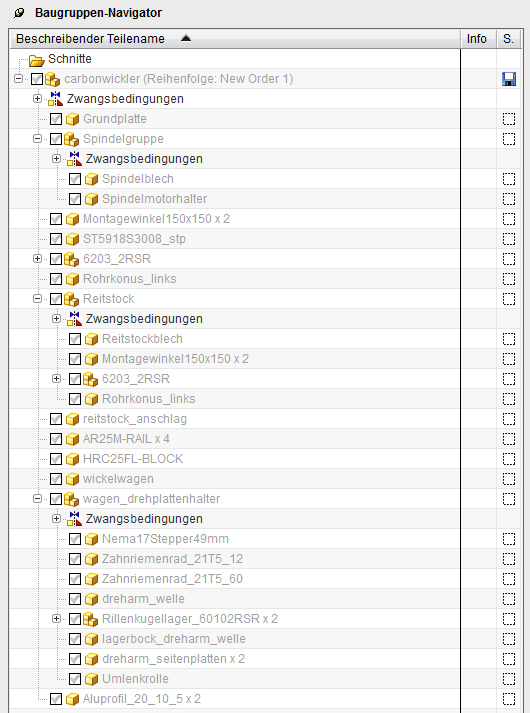
\includegraphics[width=0.4\textwidth]{NX_Screenshots/baugruppen.png}
	\caption{Übersicht über die Baugruppenstruktur} 
	\label{fig:baugruppenstruktur}
\end{figure}


Während der Konstruktion können Variablen festgelegt werden die Bauteilübergreifend verwendbar sind. Die Ausrichtung innerhalb einer Baugruppe von den einzelnen Modelle zueinander wird mit sogenannten Zwangsbedingungen festgelegt. Eine Zwangsbedingungen kann z.B. festlegen, dass sich zwei Flächen berühren soll, oder Flächen bündig ausgerichtet werden sollen. 

Ein etwas spezielleres Feature das man nutzen kann sind sogenannte Wavelinks. Dabei können beispielsweise Konturen oder Kreise von einem Modell in ein anderes verknüpft werden und sind dort weiterverwendbar. Praktisch ist dies z.B. bei Bohrungslöcher für Schrauben, wobei die Position der Bohrungslöcher zueinander von einem anderen Modell übernommen wurde. Ist diese Verknüpfung assoziativ werden auch künftige Änderungen an dem Ursprungsmodell im verknüpften Modell übernommen.
    
\section{Konzept}
Der Grundaufbau der Wickelmaschine gleicht dem einer Drehbank. Es gibt eine Drehachse die den Wickelkörper rotiert, sowie einen Arm der auf einer Achse längs dem Wickelkörper bewegt wird. Dieser Arm führt den Roving und sorgt für eine exakte Platzierung, weshalb der Arm zusätzlich senkrecht zur Wickelachse bewegbar und rotierbar ist. Auf diese Weiße lässt sich der Abstand zwischen Wickelkörper und Arm varrieren sowie die Orientierung an den aktuellen Wickelwinkel anpassen. Zur Ansteuerung der Achsen kommen Schrittmotoren zum Einsatz, da diese zum einen vergleichsweise einfach und kostengünstig ansteuerbar sind und zum andern fertige Module mit Steppertreibern verfügbar sind. Über den oben beschriebenen drehbaren Arm wird der Roving zum Wickelkörper geführt, wobei dieser zuvor mit Epoxydharz getränkt werden muss, da dies je nach Gewebedicke nach dem Wickeln nur schlecht möglich ist. Außerdem ist durch die vorgesehene automatische Tränk- und Abstreifvorrichtung eine gleichmäßige Harzmenge garantiert. Durch eine variable Positionierung des Reitstocks sind Wickelkörper in fast beliebigen Längen und Durchmessern, bis zu \SI{1200}{\milli\metre} Länge und unter \SI{250}{\milli\metre} Durchmesser, möglich.

\section{Mechanik}
Der mechanische Aufbau der Wickelmaschine ist in Siemens NX modelliert. Manche Details wie Schrauben wurden dabei an irrelevanten Stellen weggelassen. Das Augenmerk liegt insbesondere auf den Teilen die in der Fräse selbst herzustellen sind, wie z.B. die Motorhalterungen, der Reitstock und die Verbindungen zu Teilen wie den Schrittmoten. Außerdem lässt sich in dem Maschinenmodell überprüfen, dass die Verbindungen und Lage der verschiedenen Teile zueinander stimmt. Im folgenden sollen die einzelnen Teile der Wickelmaschine näher betrachtet und erklärt werden.

\subsection{Grundplatte}
Die Grundplatte dient als Aufnahme für die weiteren Teile wie Spindel, Reitstock, Linearführunen usw. Aus Kosten- und Gewichtsgründen wird diese aus Multiplexplatte hergestellt, weil die Festigkeit für die zu erwartende geringe mechanische Belastung ausreichend ist. Auf Ihr müssen Spindelhalter, Reitstock und die lange Linearführung montiert werden. Der Reitstock ist dazu noch verschiebbar, um die Maschine auf verschieden lange Wickelkörper anpassen zu können.

\subsection{Spindel}
Die Spindel nimmt eine Seite des Wickelkörpers auf und treibt diesen mithilfe eines Schrittmotors an. Die Aufnahme für den Wickelkörper ist Kegelförmig um unterschiedlich große Rohrdurchmesser von innen Spannen zu können. Die Kraftübertragung geschieht über Reibung bei bei einer Drehbank, in der Material zwischen Spitzen gespannt ist. Für spezielle Wickelkörper ist der Kegel zusätzlich noch austauschbar. In der Achsenbeschreibung hat diese Achse den Buchstaben C, also parallel zur linearen Achse Z gelegen.

\begin{figure}[H]
	\centering
	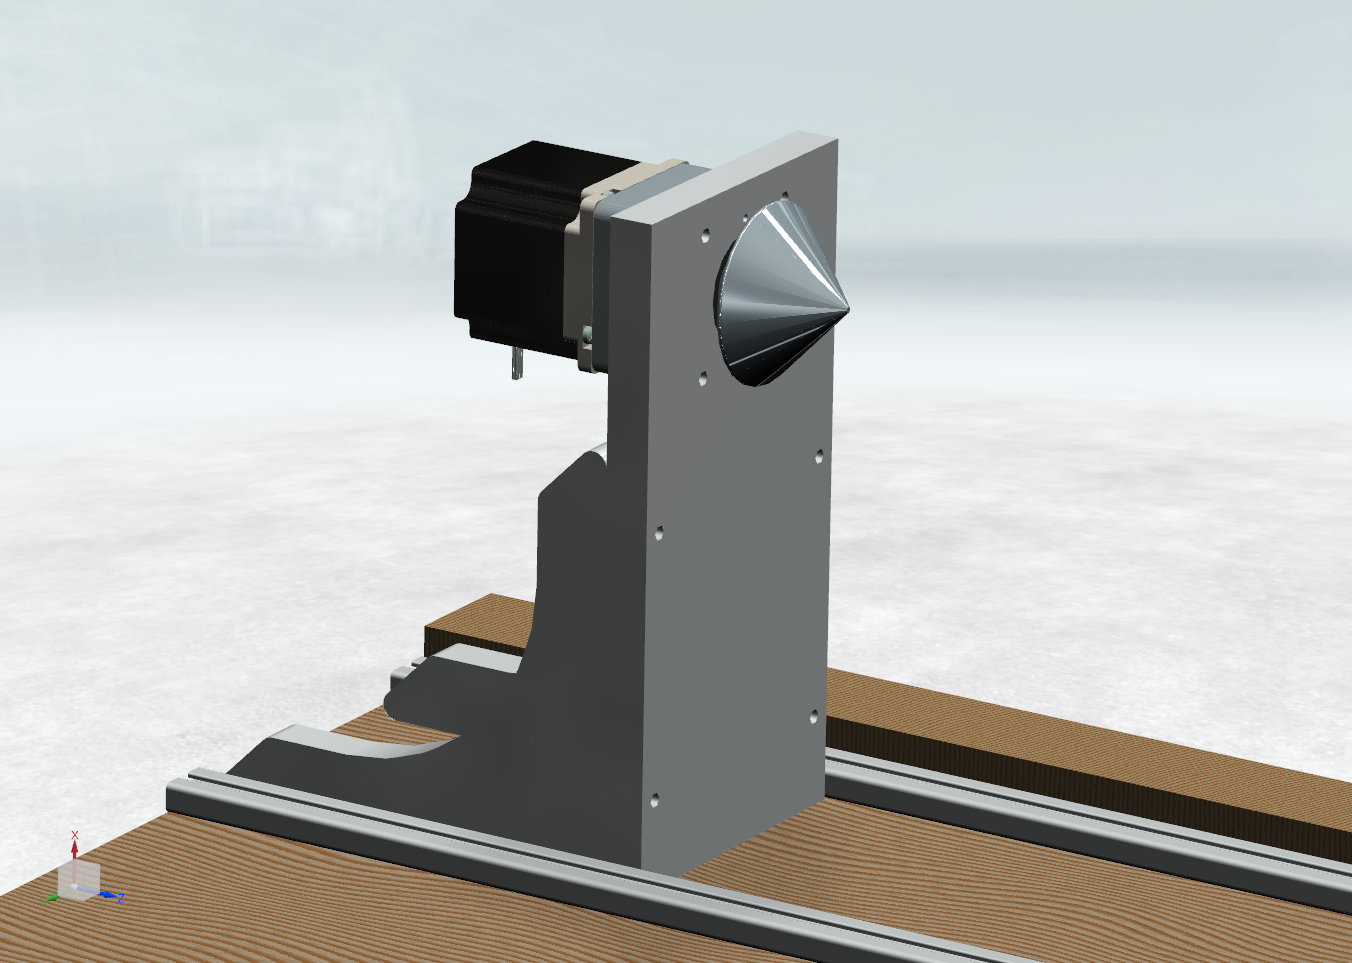
\includegraphics[width=0.8\textwidth]{NX_Screenshots/spindel.png}
	\caption{angetriebene Spindel inkl. Halterung und Aufnahmekegel} 
	\label{fig:spindel}
\end{figure}

\subsection{Reitstock}
Am Reitstock wird der Wickelkörper leicht drehbar gegengelagert. Um unterschiedlich lange Wickelkörper verwenden zu können ist dieser in Z-Richtung stufenlos verschiebbar. Der Aufbau ist ähnlich dem der Spindel mit Ausnahme des fehlenden Antriebs. Zusätzlich ist eine Feder vorgesehen die den Kegel auf den Wickelkörper drückt. Dies ermöglicht ein einfacheres Wechseln des Wickelkörpers, ohne den Reitstock selbst verschieben zu müssen.


\subsection{Wickelwagen}
Der Wickelwagen lagert auf einer langen Linearführung und führt den eigendlichen Wickelvorgang aus. Da darauf später nicht wenig Gewicht lagert, muss er robust ausgeführt und gegen Verkippen gesichert sein. Wir haben uns entschieden, eine Linearführung mit aufgesetztem Wagen zu kaufen und nicht auf sonst im Hobbybereich anzutreffende unterstützte Wellen oder Schubladenschienen zurückzugreifen.\\
Der Wagen führt demnach die Bewegung in der Achse Z aus und trägt eine weitere, kleine Linearführung, die dann die Bewegung in X-Richtung ermöglicht. Damit entspricht der Wagen dem Planschlitten einer Drehbank. Die folgenden Abbildungen zeigen die verwendeten Linearführungen.

\begin{figure}[H]
	\centering
	\includegraphics[width=0.8\textwidth]{bilder/IMG_2616.JPG}
	\caption{Linearführungen im demontierten Zustand} 
	\label{fig:wagen}
\end{figure}

\begin{figure}[H]
	\centering
	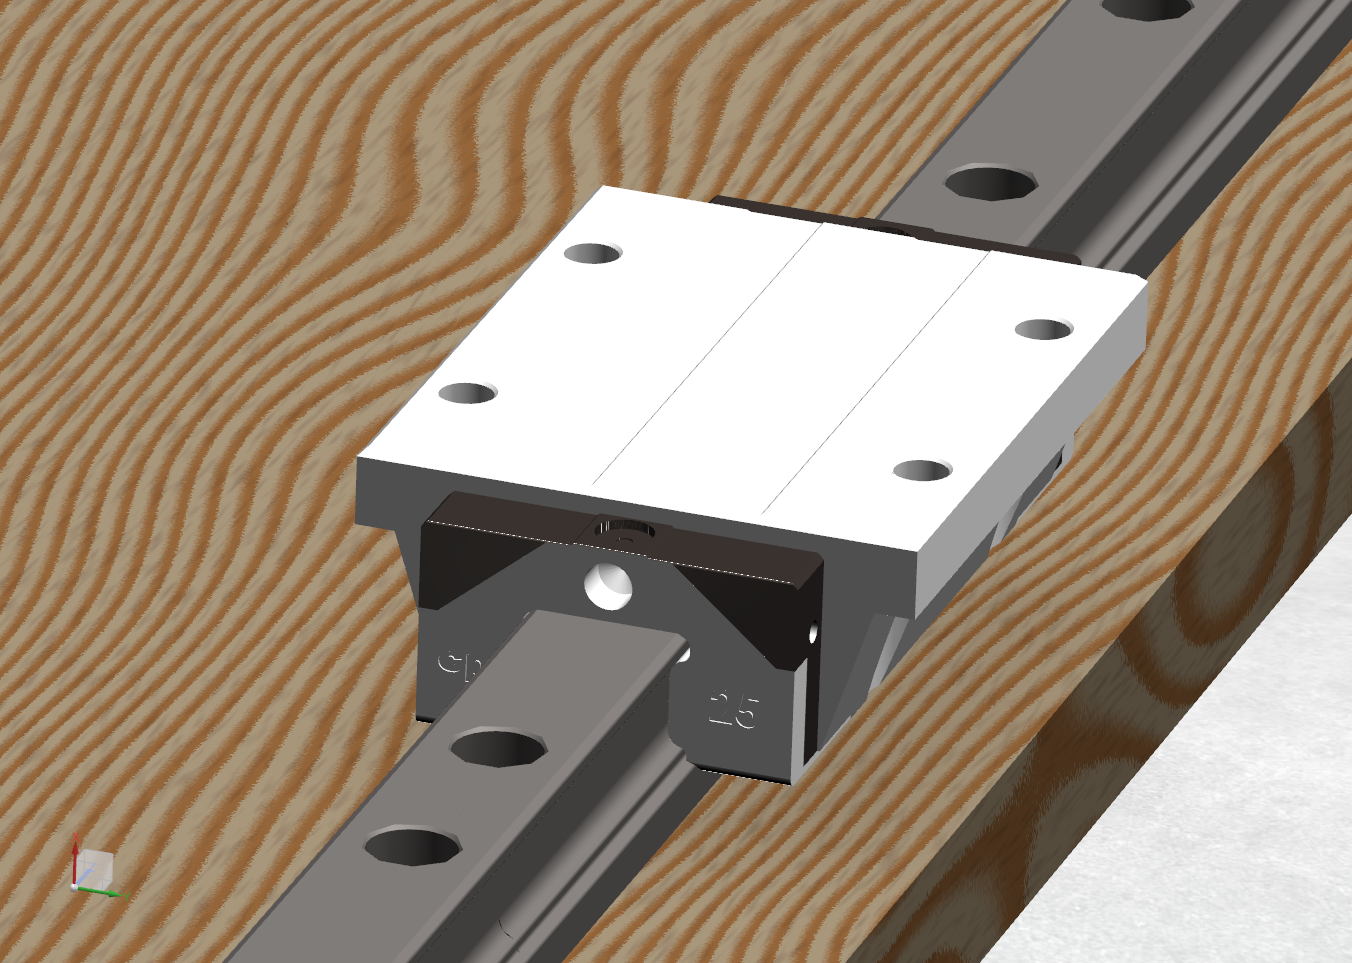
\includegraphics[width=0.8\textwidth]{NX_Screenshots/wagen.png}
	\caption{Wagen der Linearführung in NX} 
	\label{fig:wagen_foto}
\end{figure}


\subsection{Dreharm}
\begin{figure}[H]
	\centering
	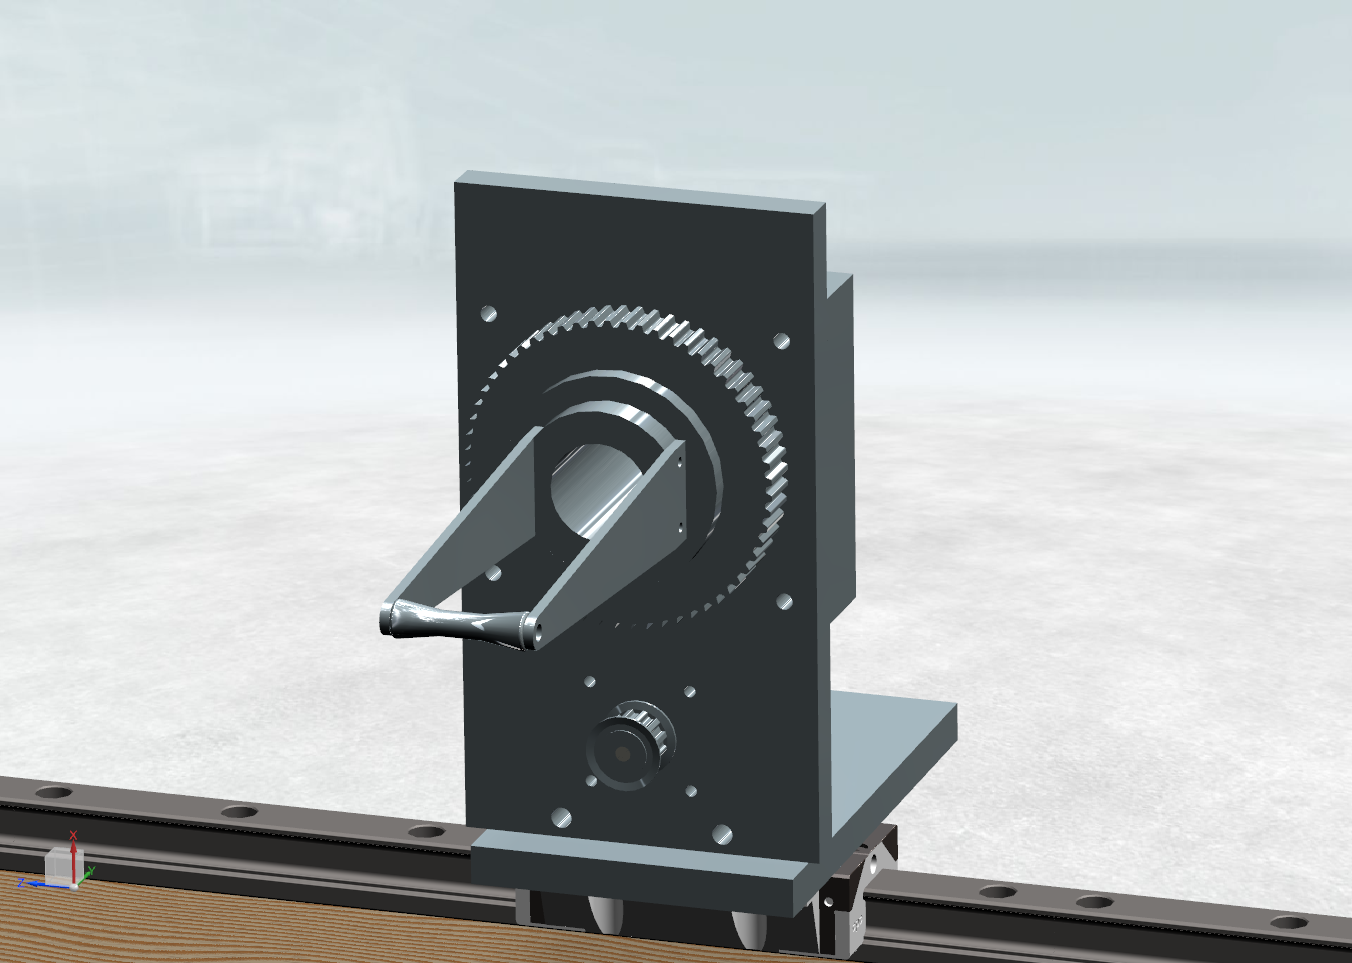
\includegraphics[width=0.8\textwidth]{NX_Screenshots/arm_vorne.png}
	\caption{Dreharm mit Rovingführung} 
	\label{fig:dreharm}
\end{figure}
Hier sieht man die Adapterplatte, die auf dem Wickelwagen (unten in der Mitte) befestigt wird. Das senkrechte Blechstück trägt dann einen weiteren Schrittmotor und den Rovingdurchlass mit der Dreheinheit. Diese sorgt dafür, dass auch bei komplexeren Wickelgeometrien, wie beispielsweise Flaschen oder unterschiedlich dicken Gegenständen, der Roving stets in Normalenrichtung auf das Werkstück geführt werden kann. Auf einer CNC-Maschine wäre dies die zur X-Achse parallele Drehachse, die dann mit dem Buchstaben A bezeichnet wird. Da der Roving zum Zeitpunkt des Wickelns schon mit Harz getränkt ist, müssen alle Teile, die mit dem Roving in Berührung kommen, aus Teflon hergestellt werden. Hier trifft das auf die kleine, leicht zylindrische Rolle vorn am Drehaufsatz zu, diese wird durch zwei Schrauben gehalten und ist so leicht ausbaubar oder sogar austauschbar.\\
Der Antrieb der X-Achse ist hier auch ausgeblendet, um die Drehvorrichtung der Achse A besser zeigen zu können.


\subsection{Tränkeinheit}
Bevor das Roving auf den Wickelkörper aufgebracht werden kann muss es zuerst mit Harz getränkt werden. Zu diesem Zweck ist ein Gefäß vorgesehen, das auf dem Wagen in Z und X Richtung mitfährt und mit einer ausreichenden Menge an Harz gefüllt ist. Dabei wurde darauf geachtet, dass möglichst wenig Harz in dem Behälter verbleibt und verschwendet wird. Im wesentlichen läuft das Roving in der Tränkeinheit über zwei Umlenkungen und einen Abstreifer an dem das überschüssige Harz entfernt und dem Behälter wieder zugeführt wird. Anschließend läuft das Roving nur noch durch den Dreharm und dessen Umlenkrolle aus Teflon um die Anzahl der zu reinigenden Teile gering zu halten.
\begin{figure}[H]
	\centering
	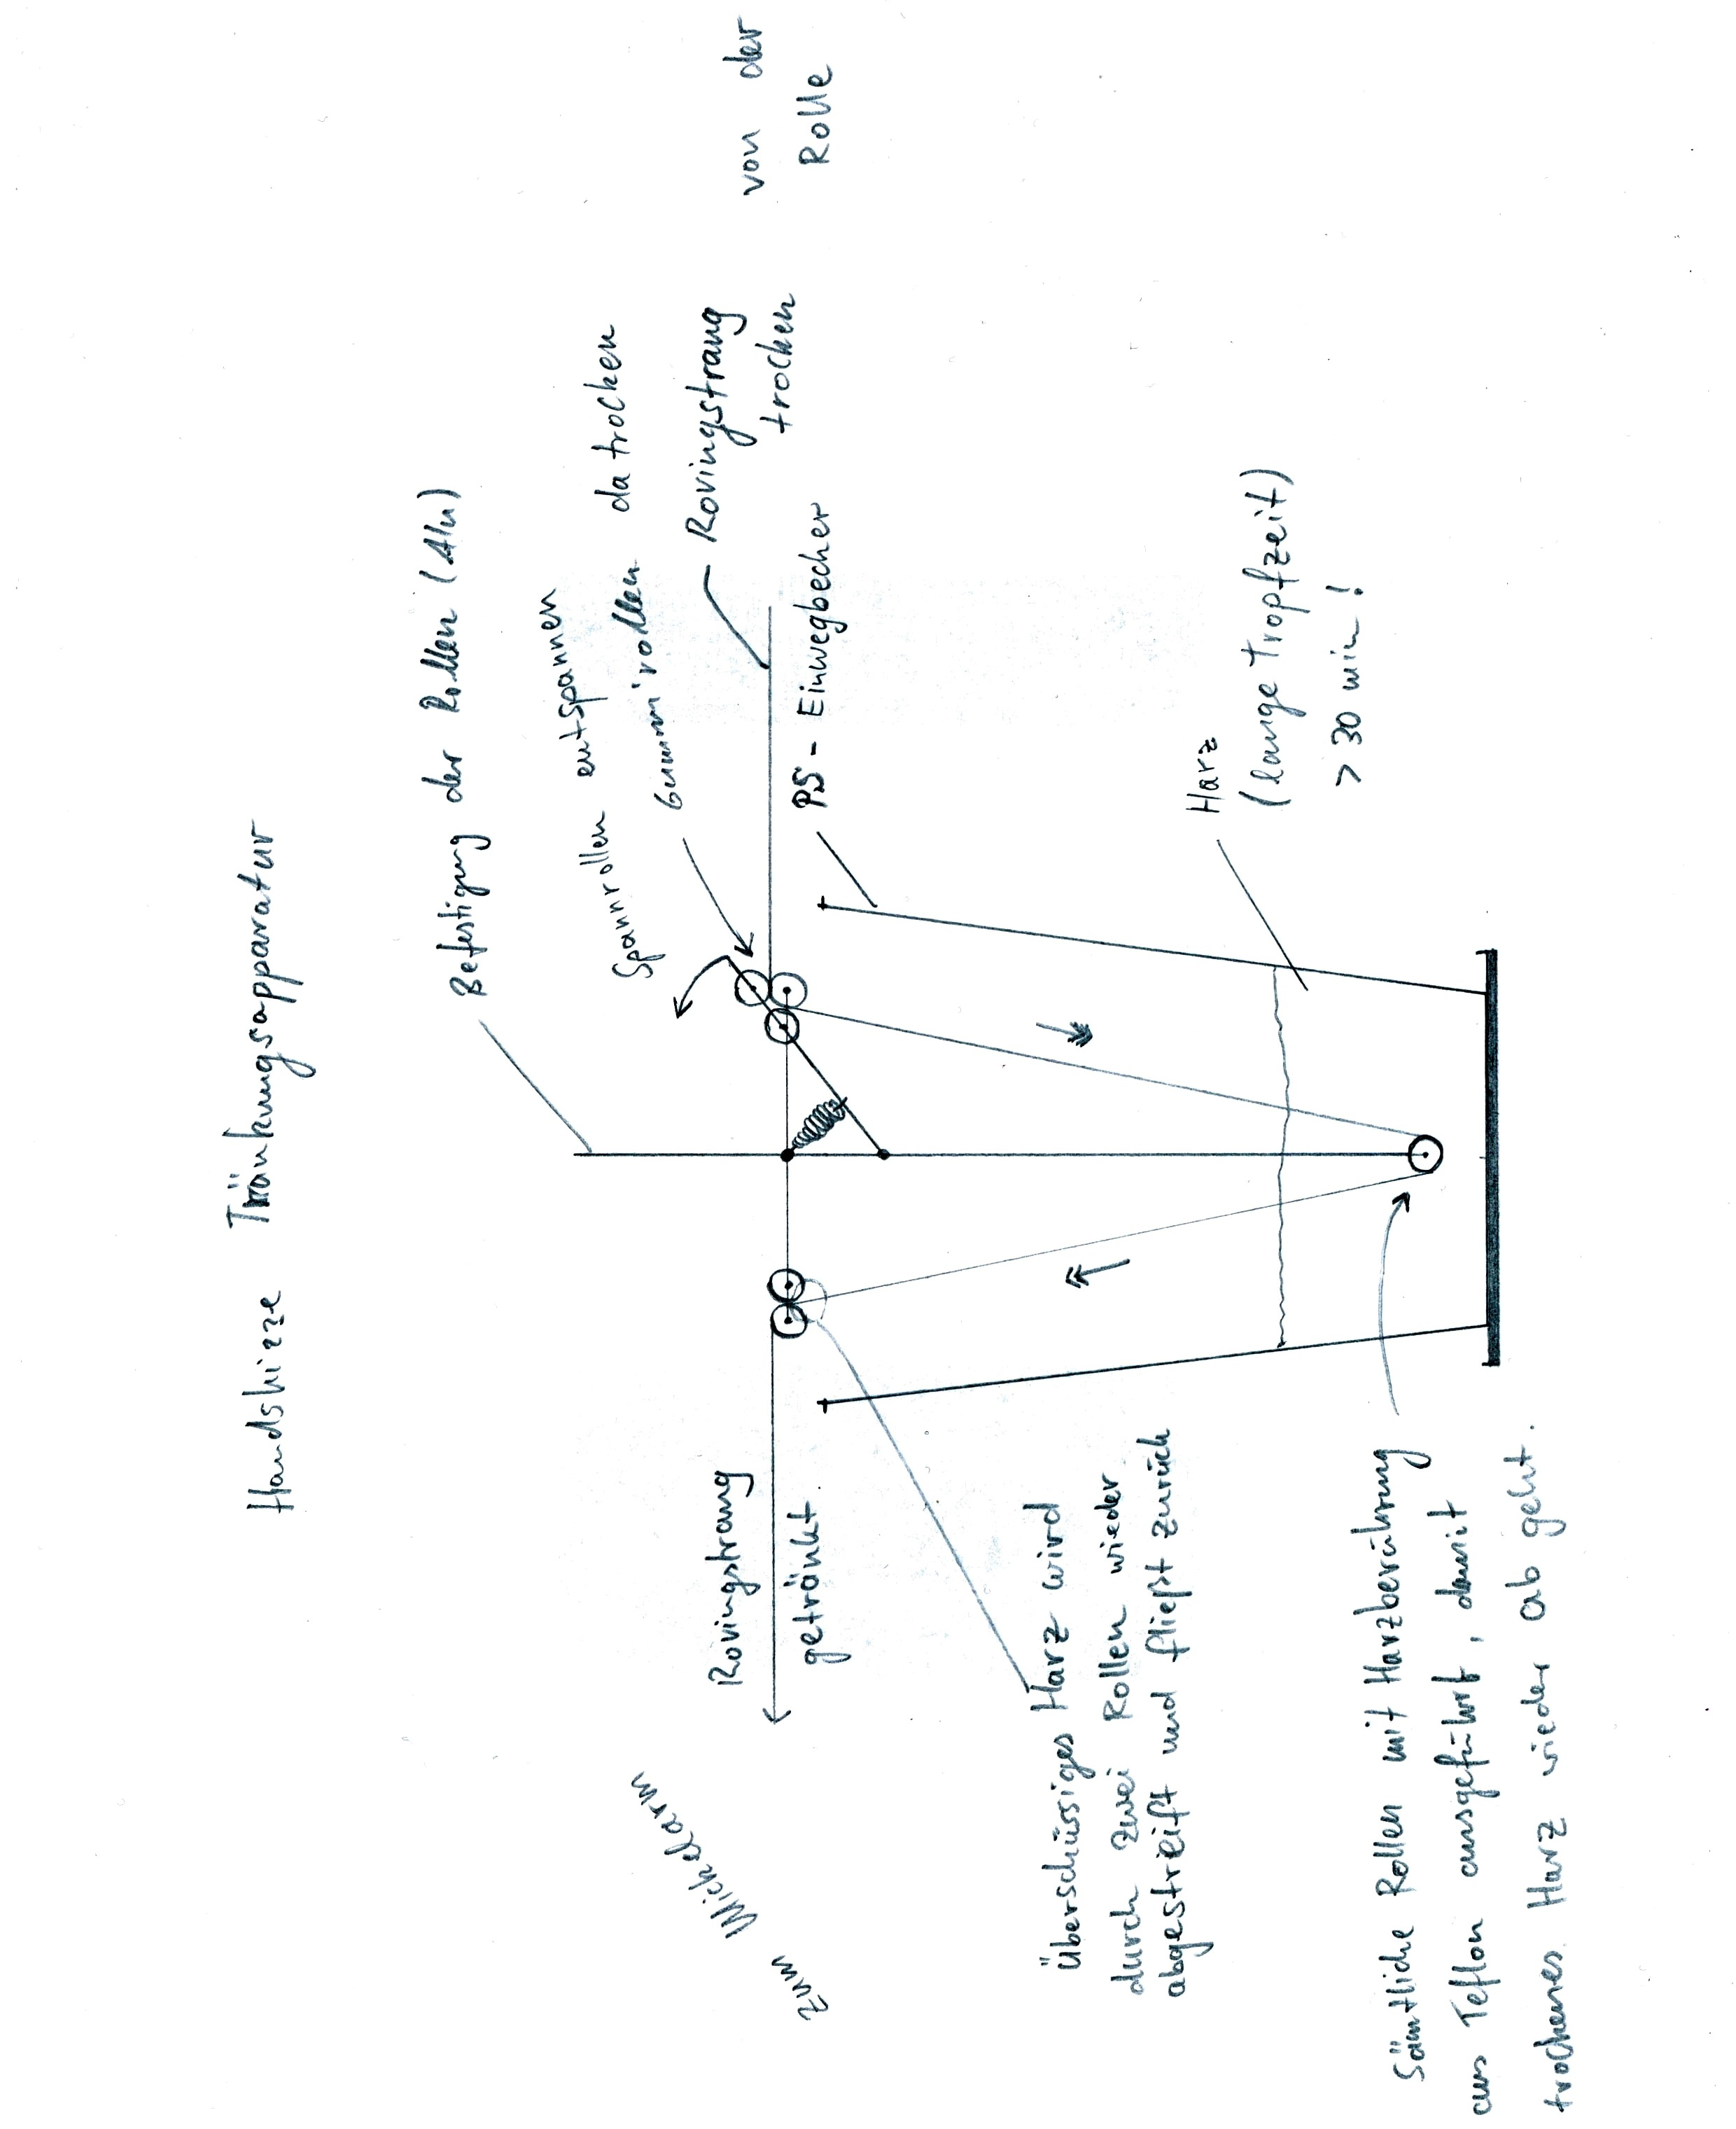
\includegraphics[angle=270, width=1\textwidth]{bilder/skizze.jpg}
	\caption{Skizze der Tränkeinrichtung} 
	\label{fig:123}
\end{figure}



\section{Software}
Die verwendete Software besteht aus zwei Teilen die im folgenden näher beschrieben werden. Zum einen einem Programm zur G-Code Erzeugung, zum anderen einem Interface zur Maschinensteuerung.
\subsection{G-Code Erzeugung}
\label{software}
Die Steuerung der Wickelmaschine erfolgt über normale G-Code Kommandos wie sie auch bei vielen anderen CNC-Maschinen verwendet werden. Für Fräs- und Drehmaschinen gibt es zur Erzeugung von G-Code anhand eine CAD Modells bereits viele Programme, für Wickelmaschinen leider nur sehr wenige und noch dazu sehr teure. Deshalb wurde auf Basis der unter \ref{mathematik} beschriebenen mathematischen Modells eine PC-Software in C++ entwickelt die  Anhand der eingestellten Parameter passenden G-Code erzeugt. In Abbildung \ref{fig:g-code} ist das graphische Userinterface zu sehen. 
\begin{figure}[H]
	\centering
	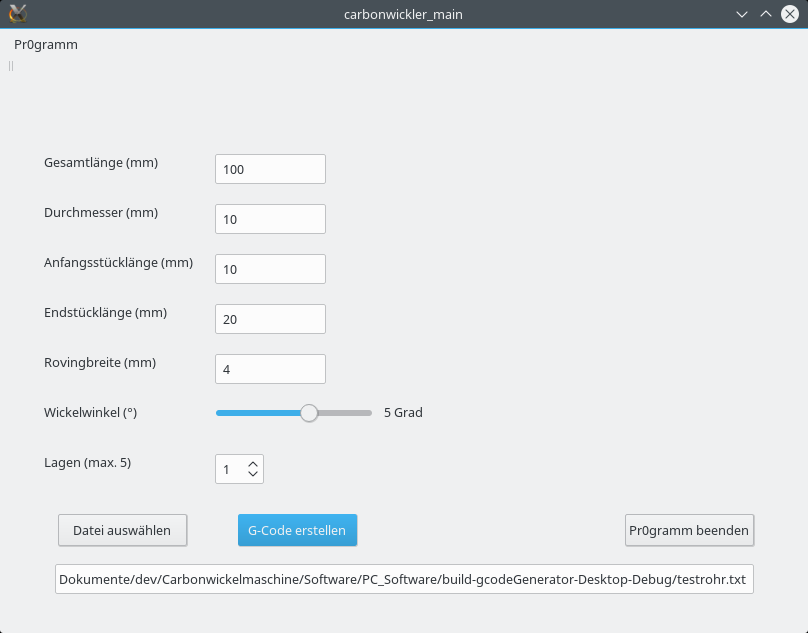
\includegraphics[width=1\textwidth]{bilder/carbowickler_software.png}
	\caption{Programm zur G-Code Erzeugung} 
	\label{fig:g-code}
\end{figure}


\subsection{grbl Interface}
Die verwendete Steuerung basiert auf grbl\cite{grbl}, welche bis zu vier Schrittmotoren anhand von G-Code ansteuert. Zum Übertragen bzw. streamen des G-Codes an die Steuerung existieren bereits mehrere fertige Programme die eingesetzt werden können, weshalb es nicht nötig ist hierfür ein neues zu entwickeln. Stattdessen ging es primäre darum G-Code zu erzeugen der zu dem gewünschten Wickelmuster führt, siehe hierzu \ref{software}. Die Hardware der Steuerung ist in \ref{fig:grbl_board} zu sehen.
\begin{figure}[H]
	\centering
	\includegraphics[width=0.8\textwidth]{bilder/IMG_2608.JPG}
	\caption{grbl-board mit stepsticks} 
	\label{fig:grbl_board}
\end{figure}

\newpage
\printbibliography

\end{document}